\begin{figure*}[p]
\centering
\begin{subfigure}[t]{\columnwidth}
  \centering
  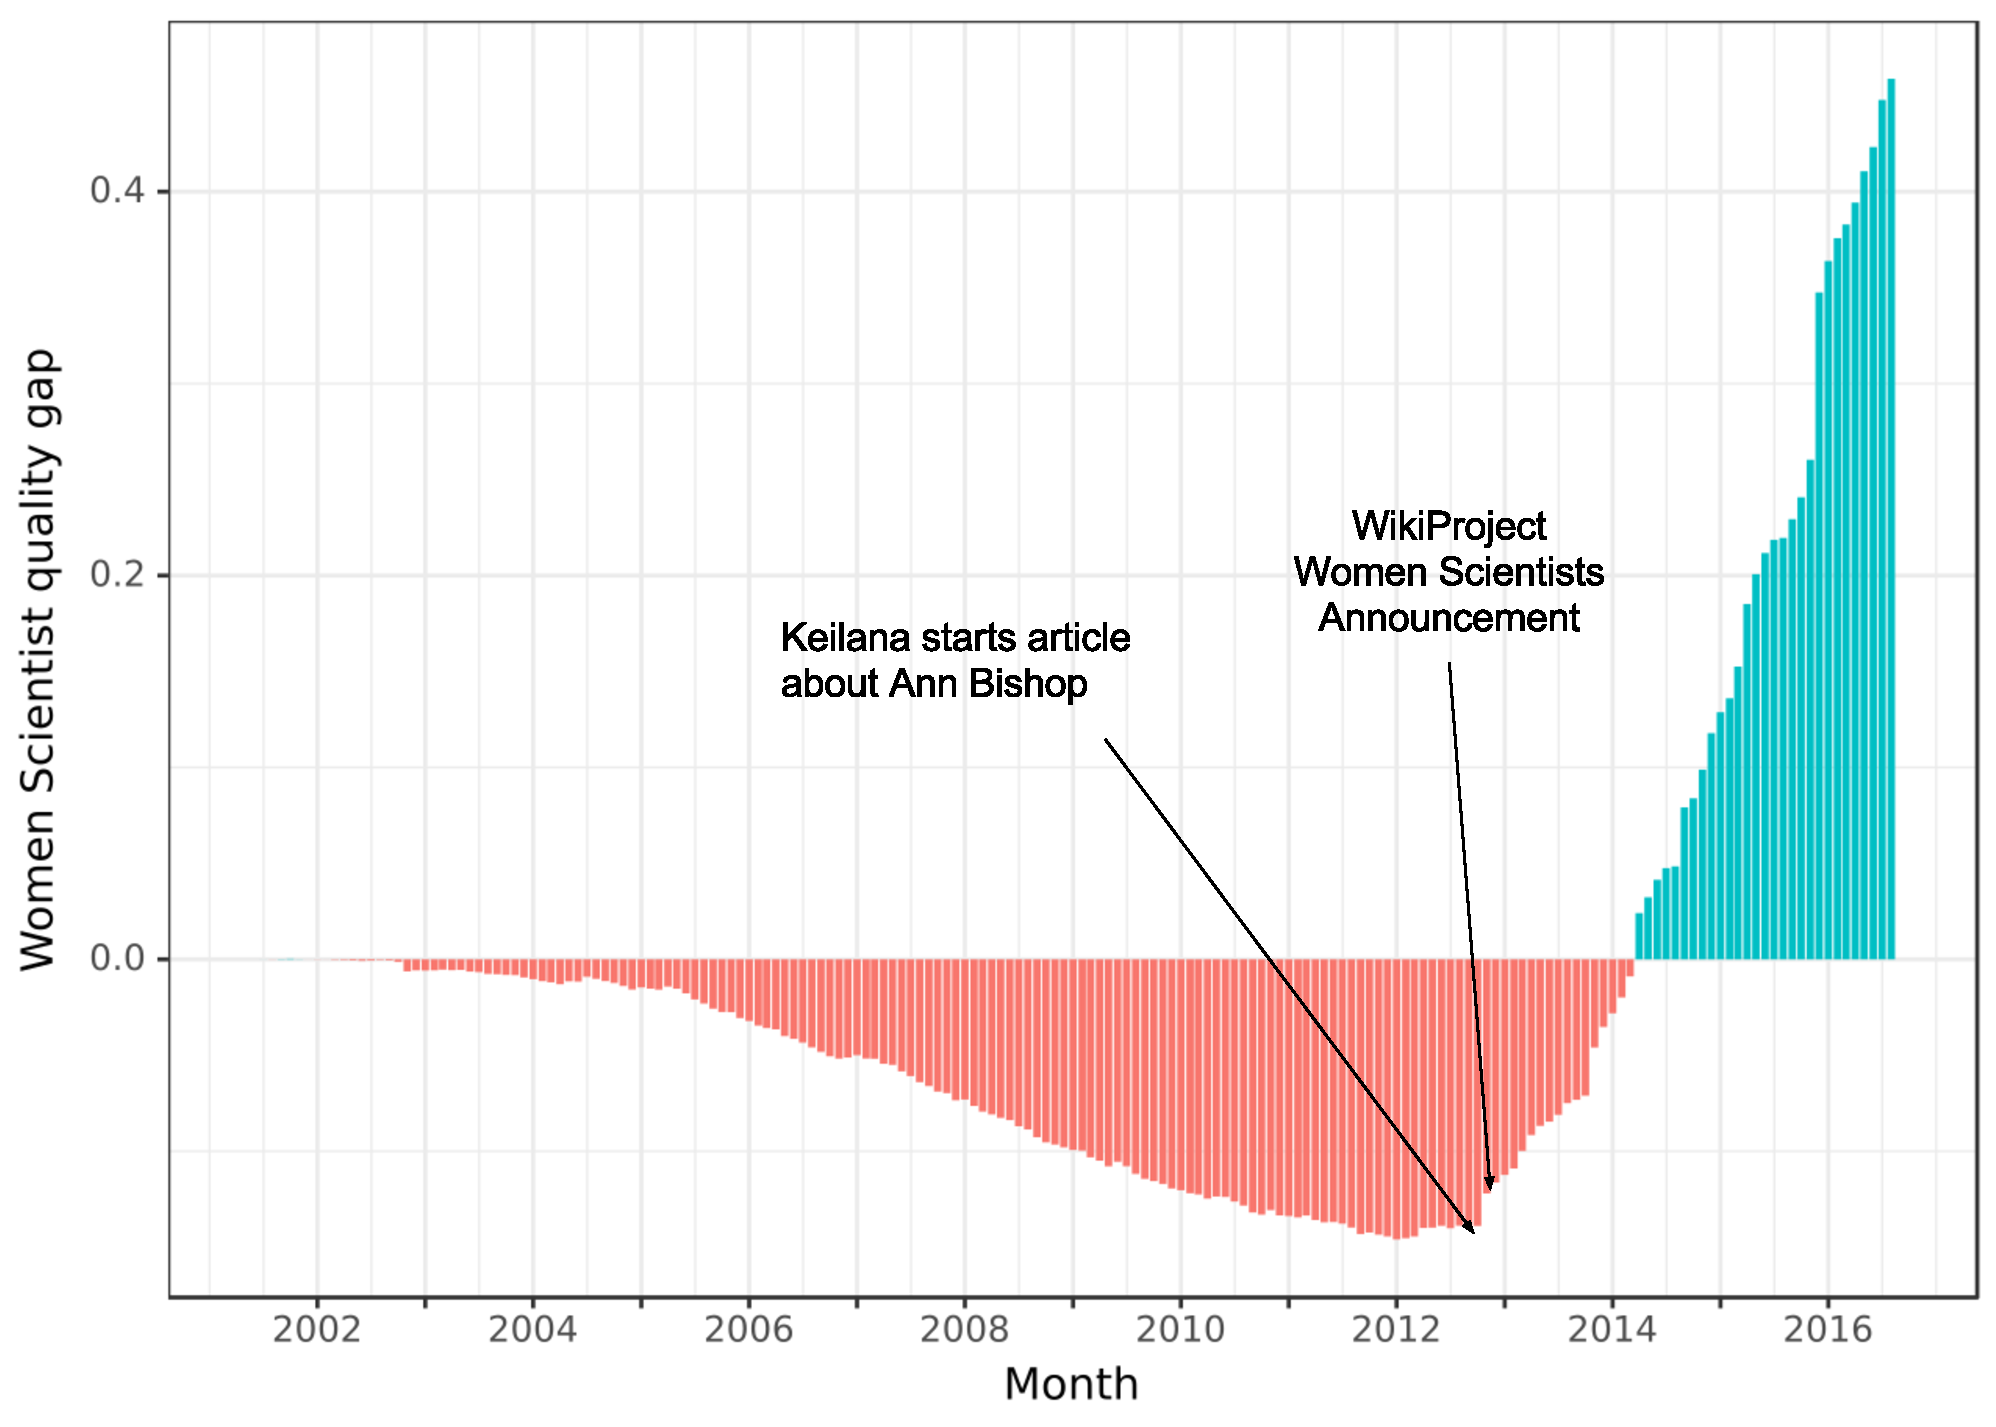
\includegraphics[width=.9\textwidth]{figures/mean_weighted_sum_ws_vs_all}
  \caption{The difference in \emph{mean weighted sum} quality predictions for all wiki and articles about Women Scientists is plotted over time. Note the transition from red to blue represents the switch from a gap to a surplus.  Important dates for User:Keilana's initiatives are annotated with arrows.}
  \label{fig:mean_weighted_sum_ws_vs_all}
\end{subfigure}\\
\begin{subfigure}[t]{\columnwidth}
  \centering
  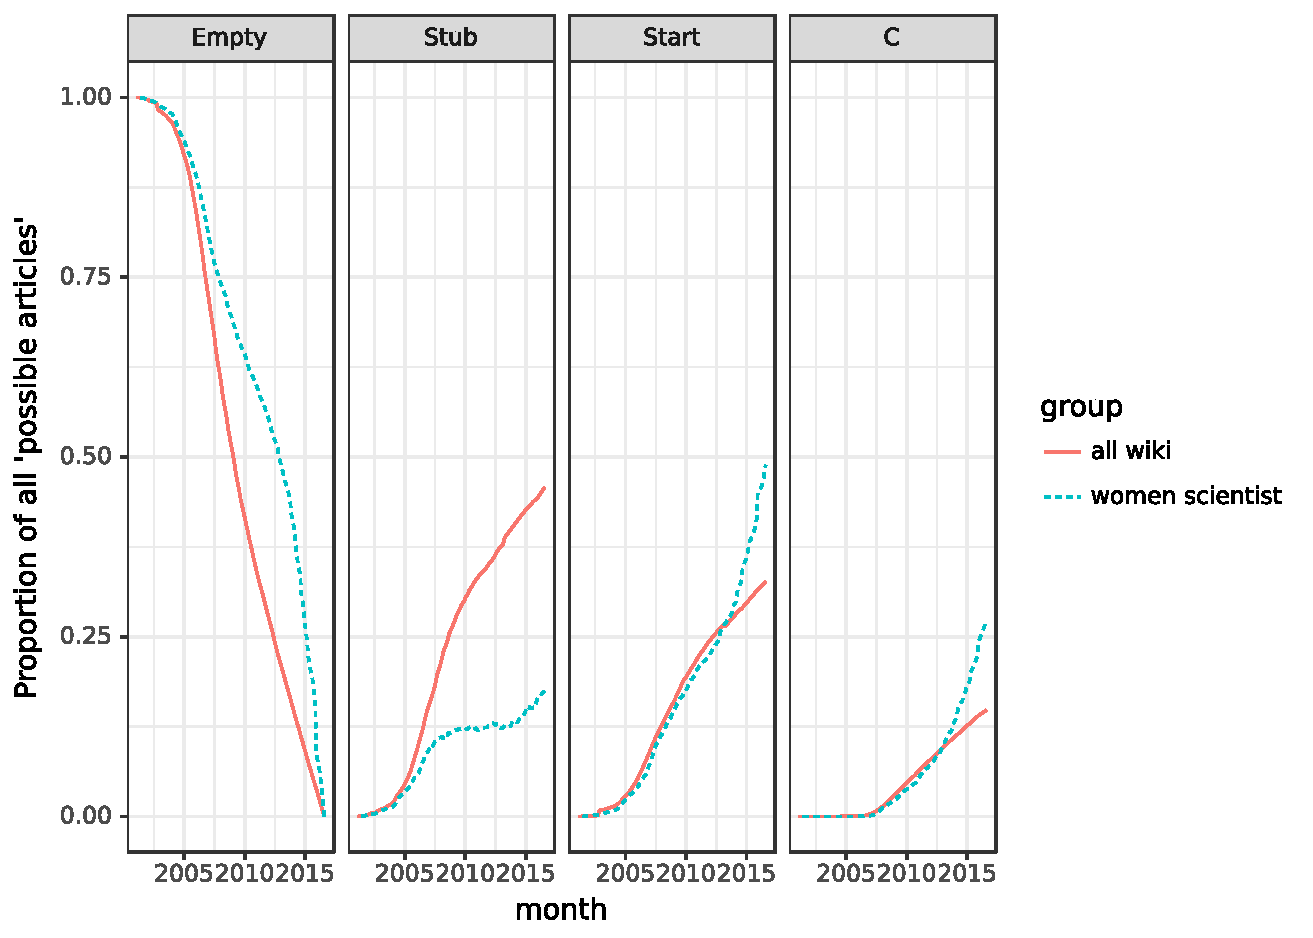
\includegraphics[width=.9\textwidth]{figures/proportion_empty2c_ws_vs_all}
  \caption{The proportion of articles falling into Empty, Stub, Start, and C-class predictions is plotted for articles tagged by WikiProject Women Scientists and all of Wikipedia.}
  \label{fig:proportion_empty2c_ws_vs_all}
\end{subfigure}~~
\begin{subfigure}[t]{\columnwidth}
  \centering
  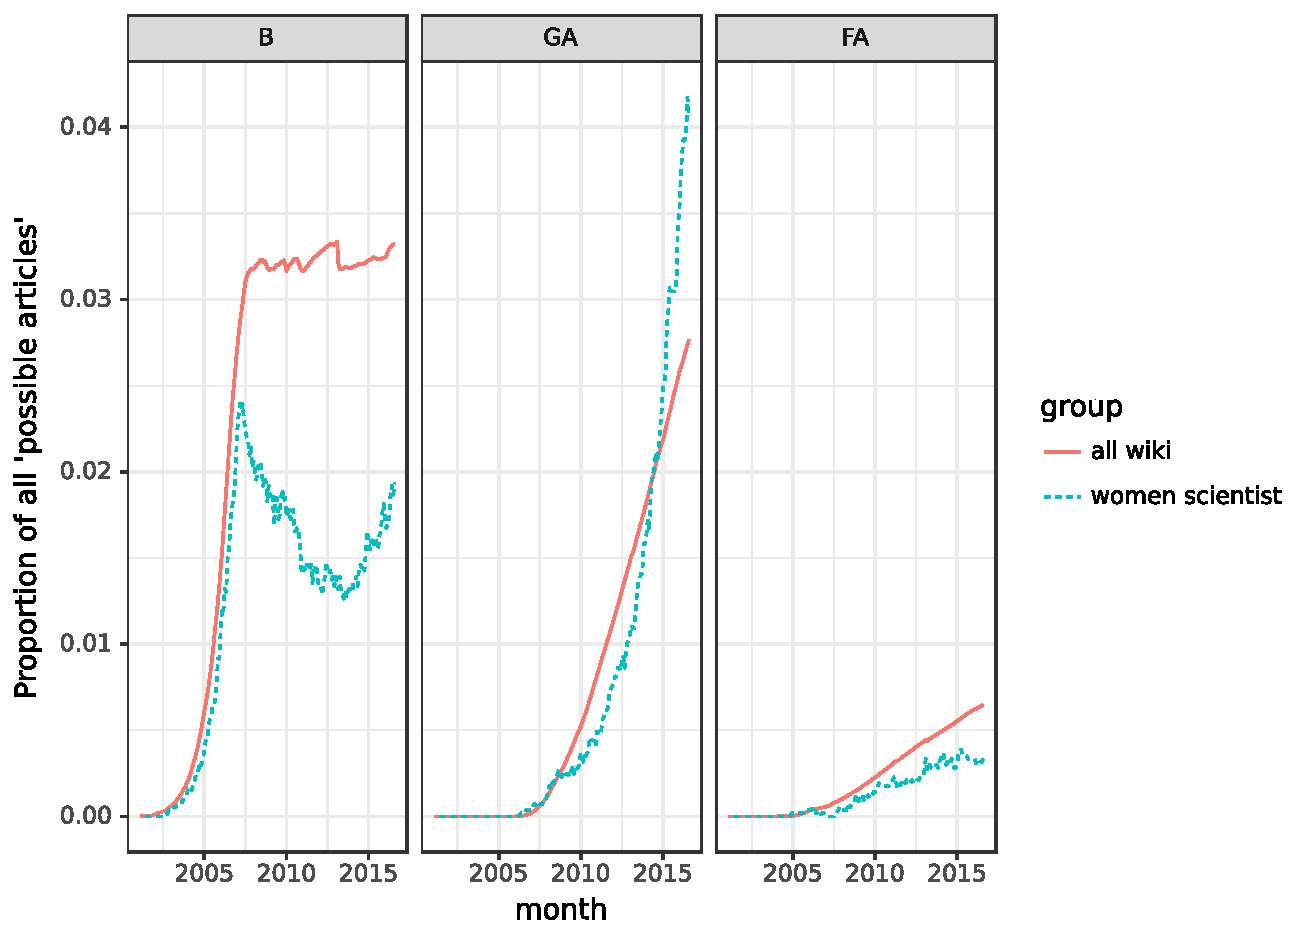
\includegraphics[width=.9\textwidth]{figures/proportion_b2fa_ws_vs_all}
  \caption{The proportion of articles falling into B, GA, and FA-class predictions is plotted for articles tagged by WikiProject Women Scientists and all of Wikipedia.}
  \label{fig:proportion_b2fa_ws_vs_all}
\end{subfigure}
\caption{The quality dynamics of biographies about women scientists vs. all of English Wikipedia.}
\label{fig:ws_vs_all}
\end{figure*}
